%% 
%% Copyright 2019-2020 Elsevier Ltd
%% 
%% This file is part of the 'CAS Bundle'.
%% --------------------------------------
%% 
%% It may be distributed under the conditions of the LaTeX Project Public
%% License, either version 1.2 of this license or (at your option) any
%% later version.  The latest version of this license is in
%%    http://www.latex-project.org/lppl.txt
%% and version 1.2 or later is part of all distributions of LaTeX
%% version 1999/12/01 or later.
%% 
%% The list of all files belonging to the 'CAS Bundle' is
%% given in the file `manifest.txt'.
%% 
%% Template article for cas-dc documentclass for 
%% double column output.

%\documentclass[a4paper,fleqn,longmktitle]{cas-dc}
\documentclass[a4paper,fleqn]{cas-dc}

%\usepackage[authoryear,longnamesfirst]{natbib}
%\usepackage[authoryear]{natbib}
\usepackage[authoryear]{natbib}

\begin{document}
\let\WriteBookmarks\relax
\def\floatpagepagefraction{1}
\def\textpagefraction{.001}
\shorttitle{PALEO-SEAL}
\shortauthors{J Drechsel et~al.}

\title [mode = title]{PALEO-SEAL: an easily deployable tool for the communication and sharing of Holocene sea-level data.}                      

\author[1]{Jan Drechsel}
\ead{jpmdrechsel@googlemail.com}
\credit{Development of the tool, work on example dataset}
\address[1]{MARUM, Center for Marine Environmental Sciences, University of Bremen, Germany}

\author[2]{Nicole Khan}
\ead{nskhan@hku.hk}
\credit{Work on database template and contribution to paper writing}
\address[2]{Department of Earth Sciences, University of Hong Kong, Hong Kong}

\author[1]{Alessio Rovere}
\cormark[1]
\ead{arovere@marum.de}
\credit{Writing of the paper, supervision on tool development}

\begin{abstract}
Lorem ipsum dolor sit amet, consectetur adipiscing elit. Nunc aliquet nunc risus, vitae porta justo semper lobortis. In tincidunt lacus nec felis dapibus, vitae vehicula elit suscipit. Nullam non lorem sed erat commodo euismod. Pellentesque non elit aliquam, dapibus ante a, commodo elit. Quisque in dignissim elit, rutrum dignissim lorem. Praesent interdum ac nibh et tempus. Donec rutrum rhoncus leo, eget egestas ex pharetra sit amet. Nulla accumsan commodo imperdiet.
\end{abstract}

\begin{keywords}
Sea-level databases \sep Visualization \sep Web interface \sep 
\end{keywords}

\maketitle

\section{Introduction}
The standardization of data on Holocene sea-level proxies has been a recurrent theme in coastal Quaternary Science research. While it was theorized and implemented at least since the early 80s \citep{shennan1982,shennan1983,VanDePlassche1986}, only recent works have established a comprehensive framework for the standardization of sea-level data and applied it globally \citep{khan2019}. The sea-level data standardization efforts were elicited by different IGCP (International Geological Correlation Programme, later renamed as the International Geoscience Programme) projects and the INQUA-PAGES project PALSEA (Palaeo-Constraints on Sea-Level Rise). 

A paper stemming from the PALSEA community \citep{dusterhus2016} highlights that the key elements to be considered when compiling a sea-level database are: Accessibility, Transparency, Trust, Availability, Continuity, Completeness, and Communication of
content. This set of properties was abbreviated into the ATTAC\textsuperscript{3} acronym. ``Communication of content'',  according to \citet{dusterhus2016}, means that interfaces for visualization, and standardized protocols for data extraction need to be implemented in order to allow users from different disciplines to easily visualize and export data of interest. 

In this short note, we present one tool designed to meet such criteria, called PALEO-SEAL. The tool makes use of a mySQL version of the sea-level data template of \citet{khan2019}. Installed on any web server supporting PHP and with few simple steps to set it up, it can be used to create a webpage to explore, plot and download Holocene sea-level data. 

\section{PALEO-SEAL description}
The core of PALEO-SEAL are two main data visualization options. One is a map, where points are clustered and de-clustered at different zoom levels. Within the map, data can be filtered either by a drop-down menu or directly on the map. The drop-down menu allows to select between: data type (type of sea-level indicator), Region, Subregion, Reference, Publication year, or Dating method. On the map, data can be filtered geographically with a ``draw rectangle'' tool (Figure \ref{fig:1}). Once a subset of data is selected, it is possible to visualize it in a data explorer interface (Figure \ref{fig:2}). The data explorer interface is composed by an age/elevation graph (with adjustable X and Y axes) and a simplified table that previews the sea-level data plotted. 

The data explorer interface has the same data filtering options as the map, and the two interfaces are linked: what is selected on the map will appear in the data interface and vice-versa. From both map and data explorer, it is possible to create a list of dataponits to be exported. Once filtering is over, an ``Export'' button allows to download the selected data as a *.csv file, compliant with the \citet{khan2019} template.

\begin{figure*}
	\centering
	
\includegraphics[width=0.8\textwidth]{figs/Figure1.png}
	\caption{}
	\label{fig:1}
\end{figure*}

\begin{figure*}
	\centering
	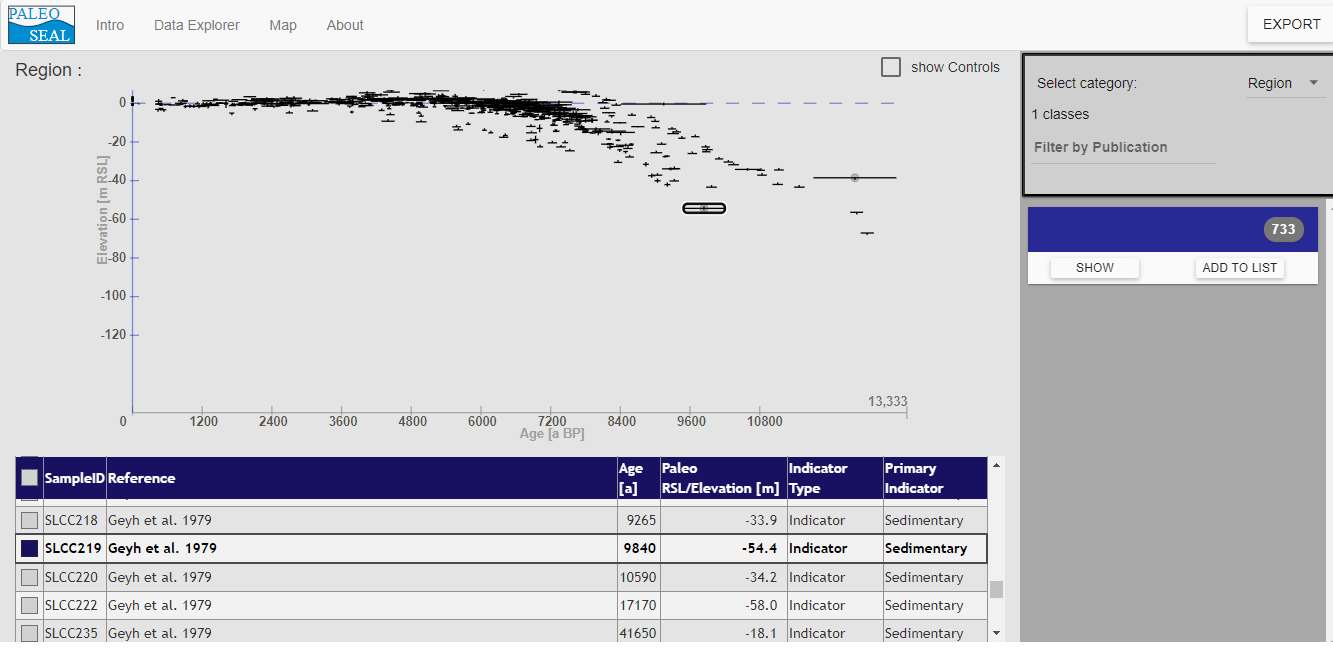
\includegraphics[width=0.8\textwidth]{figs/Figure2.png}
	\caption{}
	\label{fig:2}
\end{figure*}

\section{Installing PALEO-SEAL}
Pre-requisites for PALEO-SEAL are a server with mySQL (where data is stored) and PhP 7 installed. Then, the following steps must be followed.

\begin{enumerate}
\item \textbf{Prepare and deploy the mySQL database}. The data that will be shown in PALEO-SEAL need to be hosted on a remote server, where you will have to create a mySQL database. The only privileges needed by the interface are "SELECT" and "SHOW VIEW". As the user name will be visible to anyone with access to the code, is is strongly suggested to create a user with only these minimal privileges dedicated to the PALEO-SEAL interface. Once the database is created, run the SQL command "create table", included in the mysql folder. This will create 79 fields, reproducing the HOLSEA data table in the mySQL database. Fields headers in the database are coded with alphanumeric codes, corresponding to the fields in the HOLSEA database. To obtain descriptions of each field, you can refer to the ``$data\_headers\_lookup$'' file in the ``$data/lookups$'' folder. Then, data can be imported into the mySQL database using common import functions from csv or excel.

\item \textbf{Modify the connection string}. Navigate to ``scripts /data /connect.php" and open the file with a text editor. Edit line 3 to connect to your database as follows inserting the server name, username, password, database and port to connect to your database.

\item \textbf{Deploy your application}. Deploy the application by copying the entire PALEO-SEAL folder on a web server that supports PHP 7.0. The directory where PALEO-SEAL is copied needs to be publicly accessible.

\item \textbf{Change style (optional)}. It is possible to change the appearance of PALEO-SEAL using HTML and CSS. For example, the logo can be changed by overwriting the ``logo.svg'' file in the folder ``/ common/ img''. Webpages composing the application are contained in the folder ``/pages''. Text and content can be edited from here. To change the page style, modify the ``/ common/ css/ appearance.css'' file and, if necessary, the ``index.php'' file.
\end{enumerate}

\section{Technical details}
Jan, here 2-3 paragraphs to explain a bit the background software used to build map and xy graph.

\section{Potential use of PALEO-SEAL}
In general, PALEO-SEAL is a simple tool that can be used to illustrate, filter and make available for export Holocene sea-level data related to a paper, or a research project.   

\printcredits

%% Loading bibliography style file
%\bibliographystyle{model1-num-names}
\bibliographystyle{cas-model2-names}

% Loading bibliography database
\bibliography{cas-refs}

\end{document}

